\documentclass[12pt]{article}
\usepackage[paper=letterpaper,margin=2cm]{geometry}
\usepackage{amsmath,amssymb,amsfonts}
\usepackage{enumitem}
\usepackage{titling}
\usepackage{multirow}
\usepackage{xcolor}
\usepackage{float}
\usepackage{graphicx}
\usepackage{xcolor}
\usepackage[colorlinks=true, linkcolor=red]{hyperref}
\usepackage{subcaption} % For subfigures
\usepackage{adjustbox}  % For centering the bottom image
\usepackage{listings}
\usepackage{xcolor} % For setting colors
\usepackage{booktabs} % For better tables
\usepackage{threeparttable} % For table notes
\usepackage{pifont}    % for symbols

\usepackage{listings}
\usepackage{xcolor}

\definecolor{codegreen}{rgb}{0.0, 0.514, 0.325}      
\definecolor{codegray}{rgb}{0.75, 0.75, 0.75}    
\definecolor{codeblue}{rgb}{0.122, 0.467, 0.706}  
\definecolor{extraLightGray}{rgb}{0.98, 0.98, 0.98}
\definecolor{codepink}{rgb}{0.894, 0.0, 0.443}

\lstdefinestyle{mystyle}{
    backgroundcolor=\color{extraLightGray},
    commentstyle=\color{codegreen},
    keywordstyle=\color{codeblue},
    numberstyle=\tiny\color{codegray},
    stringstyle=\color{codepink},
    basicstyle=\ttfamily\footnotesize,
    breakatwhitespace=false,
    breaklines=true,
    captionpos=b,
    keepspaces=true,
    numbers=left,
    numbersep=5pt,
    showspaces=false,
    showstringspaces=false,
    showtabs=false,
    tabsize=2
}
\lstset{style=mystyle}

\setlength{\droptitle}{-6em}

\begin{document}

\begin{center}
Aprendizagem 2023\\
Homework I --- Group 003\\
(ist1107028, ist1107137)\vskip 1cm
\end{center}

\large{\textbf{Part I}: Pen and paper}\normalsize

\vspace{20pt}
\textbf{Consider the bivariate observations}

\begin{equation*}\{
    x_1 = \begin{bmatrix}
        1 \\
        0
    \end{bmatrix},
    x_2 = \begin{bmatrix}
        0 \\
        2
    \end{bmatrix},
    x_3 = \begin{bmatrix}
        3 \\
        -1
    \end{bmatrix}\}
\end{equation*}

\vspace{10pt}
\textbf{and the multivariate Gaussian mixture given by}

\[
\mathbf{u}_1 = \begin{bmatrix} 2 \\ -1 \end{bmatrix}, \quad
\mathbf{u}_2 = \begin{bmatrix} 1 \\ 1 \end{bmatrix}, \quad
\Sigma_1 = \begin{bmatrix} 4 & 1 \\ 1 & 4 \end{bmatrix}, \quad
\Sigma_2 = \begin{bmatrix} 2 & 0 \\ 0 & 2 \end{bmatrix}, \quad
\pi_1 = 0.5, \quad \pi_2 = 0.5
\]

\vspace{10pt}
\textbf{Answer the following questions by presenting all intermediary steps, and use 3 decimal places in
each.}

\begin{enumerate}
    \item \textbf{Perform two epochs of the EM clustering algorithm and determine the new parameters.}
    
    \vspace{10pt}
    \colorbox{codeblue}{\textcolor{white}{FIRST EM EPOCH}}

    \vspace{10pt}
    (1) Expectation: \textbf{\textcolor{codeblue}{E-STEP}}
        
        \vspace{10pt}
        \fbox{$x_1$}

        \vspace{10pt}
        \begin{itemize}[label=\ding{222}]
            \item Cluster $c=1$:
            \begin{equation*}
                \begin{aligned}
                    &\text{prior: } P(c=1) = \pi_1 = \mathbf{0.5} \\
                    \\
                    &\text{likelihood: } p(x_1|c=1) = \mathcal{N}(x_1| \mu_1, \sigma_1) \\
                    &= \frac{1}{(2 \cdot \pi)} \cdot \frac{1}{det(\Sigma_1)^{\frac{1}{2}}} \cdot \exp \left( -\frac{1}{2} \cdot (x_1 - \mu_1)^{T} \Sigma_1^{-1} \cdot (x_1 - \mu_1) \right)\\
                    &= \frac{1}{(2 \cdot \pi)} \cdot \frac{1}{\sqrt{15}} \cdot \exp \left( -\frac{1}{2} \cdot \left(\begin{pmatrix}
                    1\\
                    0
                    \end{pmatrix} - \begin{pmatrix}
                    2\\
                    -1
                    \end{pmatrix}\right)^{T} \cdot \begin{pmatrix}
                    4 & 1\\
                    1 & 4
                    \end{pmatrix}^{-1} \cdot \left(\begin{pmatrix}
                    1\\
                    0
                    \end{pmatrix} - \begin{pmatrix}
                    2\\
                    -1
                    \end{pmatrix}\right) \right)\\
                    &= \frac{1}{(2 \cdot \pi)} \cdot \frac{1}{\sqrt{15}} \cdot \exp \left( -\frac{1}{2} \cdot \begin{pmatrix}
                    -1 & 1\\
                    \end{pmatrix} \cdot \begin{pmatrix}
                    \frac{4}{15} & -\frac{1}{15}\\
                    -\frac{1}{15} & \frac{4}{15}
                    \end{pmatrix} \cdot \begin{pmatrix}
                    -1\\
                    1
                    \end{pmatrix} \right) = \frac{e^{-\frac{1}{3}}}{2\pi \cdot \sqrt{15}} = \mathbf{0.029}\\
                    \\
                    &\text{joint probability: } P(c=1, x_1) =  P(c=1)p(x_1|c=1) = \pi_1 \cdot \mathcal{N}(x_1| \mu_1, \sigma_1) = \mathbf{0.015}\\
                    \\
                    &\text{normalized posterior: } P(c=1|x_1) = \frac{0.015}{0.031+0.015} = \mathbf{0.326}
                \end{aligned}
            \end{equation*}

            \item Cluster $c=2$:
            \begin{equation*}
                \begin{aligned}
                    &\text{prior: } P(c=2) = \pi_2 = \mathbf{0.5} \\
                    \\
                    &\text{likelihood: } p(x_1|c=2) = \mathcal{N}(x_1| \mu_2, \sigma_2) \\
                    &= \frac{1}{(2 \cdot \pi)} \cdot \frac{1}{det(\Sigma_2)^\frac{1}{2}} \cdot \exp \left( -\frac{1}{2} \cdot (x_1 - \mu_2)^{T} \Sigma_2^{-1} \cdot (x_1 - \mu_2) \right)\\
                    &= \frac{1}{(2 \cdot \pi)} \cdot \frac{1}{\sqrt{4}} \cdot \exp \left( -\frac{1}{2} \cdot \left(\begin{pmatrix}
                    1\\
                    0
                    \end{pmatrix} - \begin{pmatrix}
                    1\\
                    1
                    \end{pmatrix}\right)^{T} \cdot \begin{pmatrix}
                    2 & 0\\
                    0 & 2
                    \end{pmatrix}^{-1} \cdot \left(\begin{pmatrix}
                    1\\
                    0
                    \end{pmatrix} - \begin{pmatrix}
                    1\\
                    1
                    \end{pmatrix}\right) \right)\\
                    &= \frac{1}{(2 \cdot \pi)} \cdot \frac{1}{\sqrt{4}} \cdot \exp \left( -\frac{1}{2} \cdot \begin{pmatrix}
                    0 & -1\\
                    \end{pmatrix} \cdot \begin{pmatrix}
                    \frac{1}{2} & 0\\
                    0 & \frac{1}{2}
                    \end{pmatrix} \cdot \begin{pmatrix}
                    0\\
                    -1
                    \end{pmatrix} \right) = \frac{e^{-\frac{1}{4}}}{2 \pi \cdot \sqrt{4}} = \mathbf{0.062}\\
                    \\
                    &\text{joint probability: } P(c=2, x_1) =  P(c=2)p(x_1|c=2) = \pi_2 \cdot \mathcal{N}(x_1| \mu_2, \sigma_2) = \mathbf{0.031}\\
                    \\
                    &\text{normalized posterior: } P(c=2|x_1) = \frac{0.031}{0.031+0.015} = \mathbf{0.674}
                \end{aligned}
            \end{equation*}
        \end{itemize}
        
        \vspace{10pt}
        \fbox{$x_2$}

        \vspace{10pt}
        \begin{itemize}[label=\ding{222}]
            \item Cluster $c=1$:
                
            \begin{equation*}
                \begin{aligned}
                    &\text{prior: } P(c=1) = \pi_1 = \mathbf{0.5} \\
                    &\text{likelihood: } p(x_2|c=1) = \mathcal{N}(x_2| \mu_1, \sigma_1) \\
                    &= \frac{1}{(2 \cdot \pi)} \cdot \frac{1}{det(\Sigma_1)^\frac{1}{2}} \cdot \exp \left( -\frac{1}{2} \cdot (x_2 - \mu_1)^{T} \Sigma_1^{-1} \cdot (x_2 - \mu_1) \right)\\
                    &= \frac{1}{(2 \cdot \pi)} \cdot \frac{1}{\sqrt{15}} \cdot \exp \left( -\frac{1}{2} \cdot \left(\begin{pmatrix}
                    0\\
                    2
                    \end{pmatrix} - \begin{pmatrix}
                    2\\
                    -1
                    \end{pmatrix}\right)^{T} \cdot \begin{pmatrix}
                    4 & 1\\
                    1 & 4
                    \end{pmatrix}^{-1} \cdot \left(\begin{pmatrix}
                    0\\
                    2
                    \end{pmatrix} - \begin{pmatrix}
                    2\\
                    -1
                    \end{pmatrix}\right) \right)\\
                    &= \frac{1}{(2 \cdot \pi)} \cdot \frac{1}{\sqrt{15}} \cdot \exp \left( -\frac{1}{2} \cdot \begin{pmatrix}
                    -2 & 3\\
                    \end{pmatrix} \cdot \begin{pmatrix}
                    \frac{4}{15} & -\frac{1}{15}\\
                    -\frac{1}{15} & \frac{4}{15}
                    \end{pmatrix} \cdot \begin{pmatrix}
                    -2\\
                    3
                    \end{pmatrix} \right) = \frac{e^{-\frac{32}{15}}}{2 \pi \cdot \sqrt{15}} = \mathbf{0.005}\\ 
                    \\    
                    &\text{joint probability: } P(c=1, x_2) =  P(c=1)p(x_2|c=1) = \pi_1 \cdot \mathcal{N}(x_2| \mu_1, \sigma_1) = \mathbf{0.003}\\
                    \\
                    &\text{normalized posterior: }P(c=1|x_2) = \frac{0.003}{0.024+0.003} = \mathbf{0.111}
                \end{aligned}
            \end{equation*}

            \newpage
            \item Cluster $c=2$:
            
            \begin{equation*}
                \begin{aligned}
                    &\text{prior: } P(c=2) = \pi_2 = \mathbf{0.5} \\
                    &\text{likelihood: } p(x_2|c=2) = \mathcal{N}(x_2| \mu_2, \sigma_2) \\
                    &= \frac{1}{(2 \cdot \pi)} \cdot \frac{1}{det(\Sigma_2)^\frac{1}{2}} \cdot \exp \left( -\frac{1}{2} \cdot (x_2 - \mu_2)^{T} \Sigma_2^{-1} \cdot (x_2 - \mu_2) \right)\\
                    &= \frac{1}{(2 \cdot \pi)} \cdot \frac{1}{\sqrt{4}} \cdot \exp \left( -\frac{1}{2} \cdot \left(\begin{pmatrix}
                    0\\
                    2
                    \end{pmatrix} - \begin{pmatrix}
                    1\\
                    1
                    \end{pmatrix}\right)^{T} \cdot \begin{pmatrix}
                    2 & 0\\
                    0 & 2
                    \end{pmatrix}^{-1} \cdot \left(\begin{pmatrix}
                    0\\
                    2
                    \end{pmatrix} - \begin{pmatrix}
                    1\\
                    1
                    \end{pmatrix}\right) \right)\\
                    &= \frac{1}{(2 \cdot \pi)} \cdot \frac{1}{\sqrt{4}} \cdot \exp \left( -\frac{1}{2} \cdot \begin{pmatrix}
                    -1 & 1\\
                    \end{pmatrix} \cdot \begin{pmatrix}
                    \frac{1}{2} & 0\\
                    0 & \frac{1}{2}
                    \end{pmatrix} \cdot \begin{pmatrix}
                    -1\\
                    1
                    \end{pmatrix} \right) = \frac{e^{-\frac{1}{2}}}{2 \pi \cdot \sqrt{4}} = \mathbf{0.048}\\
                    \\
                    &\text{joint probability: } P(c=2, x_2) =  P(c=2)p(x_2|c=2) = \pi_2 \cdot \mathcal{N}(x_2| \mu_2, \sigma_2) = \mathbf{0.024}\\
                    \\
                    &\text{normalized posterior: } P(c=2|x_2) = \frac{0.024}{0.024 + 0.003} = \mathbf{0.889}
                \end{aligned}
            \end{equation*}
        \end{itemize}

        \vspace{10pt}
        \fbox{$x_3$}

        \vspace{10pt}
        \begin{itemize}[label=\ding{222}]
            \item Cluster $c=1$:
                
            \begin{equation*}
                \begin{aligned}
                    &\text{prior: } P(c=1) = \pi_1 = \mathbf{0.5} \\
                    &\text{likelihood: } p(x_3|c=1) = \mathcal{N}(x_3| \mu_1, \sigma_1) \\
                    &= \frac{1}{(2 \cdot \pi)} \cdot \frac{1}{det(\Sigma_1)^\frac{1}{2}} \cdot \exp \left( -\frac{1}{2} \cdot (x_3 - \mu_1)^{T} \Sigma_1^{-1} \cdot (x_3 - \mu_1) \right)\\
                    &= \frac{1}{(2 \cdot \pi)} \cdot \frac{1}{\sqrt{15}} \cdot \exp \left( -\frac{1}{2} \cdot \left(\begin{pmatrix}
                    3\\
                    -1
                    \end{pmatrix} - \begin{pmatrix}
                    2\\
                    -1
                    \end{pmatrix}\right)^{T} \cdot \begin{pmatrix}
                    4 & 1\\
                    1 & 4
                    \end{pmatrix}^{-1} \cdot \left(\begin{pmatrix}
                    3\\
                    -1
                    \end{pmatrix} - \begin{pmatrix}
                    2\\
                    -1
                    \end{pmatrix}\right) \right)\\
                    &= \frac{1}{(2 \cdot \pi)} \cdot \frac{1}{\sqrt{15}} \cdot \exp \left( -\frac{1}{2} \cdot \begin{pmatrix}
                    1 & 0\\
                    \end{pmatrix} \cdot \begin{pmatrix}
                    \frac{4}{15} & -\frac{1}{15}\\
                    -\frac{1}{15} & \frac{4}{15}
                    \end{pmatrix} \cdot \begin{pmatrix}
                    1\\
                    0
                    \end{pmatrix} \right) = \frac{e^{-\frac{2}{15}}}{2 \pi \cdot \sqrt{15}} = \mathbf{0.036}\\
                    \\
                    &\text{joint probability: } P(c=1, x_3) =  P(c=1)p(x_3|c=1) = \pi_1 \cdot \mathcal{N}(x_3| \mu_1, \sigma_1) = \mathbf{0.018}\\
                    \\
                    &\text{normalized posterior: } P(c=1|x_3)= \frac{0.018}{0.018+0.006} = \mathbf{0.750}
                \end{aligned}
            \end{equation*}

            \newpage
            \item Cluster $c=2$:
            
            \begin{equation*}
                \begin{aligned}
                    &\text{prior: } P(c=2) = \pi_2 = \mathbf{0.5} \\
                    &\text{likelihood: } p(x_3|c=2) = \mathcal{N}(x_3| \mu_2, \sigma_2) \\
                    &= \frac{1}{(2 \cdot \pi)} \cdot \frac{1}{det(\Sigma_2)^\frac{1}{2}} \cdot \exp \left( -\frac{1}{2} \cdot (x_3 - \mu_2)^{T} \Sigma_2^{-1} \cdot (x_3 - \mu_2) \right)\\
                    &= \frac{1}{(2 \cdot \pi)} \cdot \frac{1}{\sqrt{4}} \cdot \exp \left( -\frac{1}{2} \cdot \left(\begin{pmatrix}
                    3\\
                    -1
                    \end{pmatrix} - \begin{pmatrix}
                    1\\
                    1
                    \end{pmatrix}\right)^{T} \cdot \begin{pmatrix}
                    2 & 0\\
                    0 & 2
                    \end{pmatrix}^{-1} \cdot \left(\begin{pmatrix}
                    3\\
                    -1
                    \end{pmatrix} - \begin{pmatrix}
                    1\\
                    1
                    \end{pmatrix}\right) \right)\\
                    &= \frac{1}{(2 \cdot \pi)} \cdot \frac{1}{\sqrt{4}} \cdot \exp \left( -\frac{1}{2} \cdot \begin{pmatrix}
                    2 & -2\\
                    \end{pmatrix} \cdot \begin{pmatrix}
                    \frac{1}{2} & 0\\
                    0 & \frac{1}{2}
                    \end{pmatrix} \cdot \begin{pmatrix}
                    2\\
                    -2
                    \end{pmatrix} \right) = \frac{e^{-2}}{2 \pi \cdot \sqrt{4}} = \mathbf{0.012}\\
                    \\
                    &\text{joint probability: } P(c=1, x_3) =  P(c=1)p(x_3|c=1) = \pi_1 \cdot \mathcal{N}(x_3| \mu_1, \sigma_1) = \mathbf{0.006}\\
                    \\
                    &\text{normalized posterior: } P(c=2|x_3) = \frac{0.006}{0.006+0.018} = \mathbf{0.250}
                \end{aligned}
            \end{equation*}
        \end{itemize}


        \begin{table}[H]
            \begin{center}
                \begin{threeparttable}
                \begin{tabular}{c|c|c}
                    Observations & $c=1$ & $c=2$ \\
                    \hline
                    $x_1$ & $0.326$ & $0.674$\\
                    $x_2$ & $0.111$ & $0.889$\\
                    $x_3$ & $0.750$ & $0.250$\\
                \end{tabular}
                \caption{Normalized posteriors}
                \end{threeparttable}
            \end{center}
        \end{table}

        \vspace{10pt}
        (2) Maximization: \textbf{\textcolor{codeblue}{M-STEP}}
        
        \vspace{10pt}
        For the recalculation we will use the following formulas (n represents the cluster):

        \vspace{10pt}
        For the means:
        \begin{equation}\label{means}
            \mu_\text{n} = \frac{P(c=n|x_1) \cdot x_1 + P(c=n|x_2) \cdot x_2 + P(c=n|x_3) \cdot x_3}{P(c=n|x_1) + P(c=n|x_2) + P(c=n|x_3)}
        \end{equation}

        \vspace{10pt}
        For the covariance matrices:

        \begin{equation}\label{covariance_matrix}
            \Sigma_n = \begin{pmatrix}
                \Sigma_{11} & \Sigma_{21} \\
                \Sigma_{12} & \Sigma_{22} \\
            \end{pmatrix}
        \end{equation}
        
        Where
        \begin{equation*}
            \resizebox{0.88\hsize}{!}{$
            \Sigma_{ij} = \frac{
              P(c=n|x_1)\left(\left(x_{1i} - \mu_{ni}\right) \left(x_{1j}- \mu_{nj}\right)\right) 
            + P(c=n|x_2)\left(\left(x_{2i} - \mu_{ni}\right) \left(x_{2j}- \mu_{nj}\right)\right) 
            + P(c=n|x_3)\left(\left(x_{3i} - \mu_{ni}\right) \left(x_{3j}- \mu_{nj}\right)\right)
            }{P(c=n|x_1) + P(c=n|x_2) + P(c=n|x_3)}
            $}
        \end{equation*}
        
        \newpage
        \ding{222} Cluster $c=1$:

        \begin{equation*}
            \fontsize{8pt}{10pt}\selectfont
            \mu_1 = \frac{0.326 \cdot x_1 + 0.111 \cdot x_2 + 0.75 \cdot x_3}{0.326+0.111+0.75} = \frac{0.326 \cdot \begin{pmatrix}
            1\\
            0
            \end{pmatrix}+ 0.111 \cdot \begin{pmatrix}
            0\\
            2
            \end{pmatrix} + 0.750 \cdot \begin{pmatrix}
            3\\
            -1
            \end{pmatrix}}{1.187} = \begin{pmatrix}
            2.170\\
            -0.445
            \end{pmatrix}\\
        \end{equation*}

        \begin{equation*}
            \Sigma_1 = \begin{pmatrix}
                \Sigma_{11} & \Sigma_{21} \\
                \Sigma_{12} & \Sigma_{22}
            \end{pmatrix} = \begin{pmatrix}
                1.252 & -0.930\\
                -0.930 & 0.808
            \end{pmatrix}
        \end{equation*}

        \begin{equation*}
            \fontsize{9pt}{10pt}\selectfont
            \begin{aligned}
                \Sigma_{11} &= \frac{0.326 \cdot ((x_{11}-\mu_{11}) \cdot (x_{11} - \mu_{11}))+ 0.111 \cdot ((x_{21}-\mu_{11}) \cdot (x_{21} - \mu_{11}))+ 0.75 \cdot ((x_{31}-\mu_{11}) \cdot (x_{31} - \mu_{11}))}{1.187}\\
                &=\frac{0.326 \cdot ((1-2.170)(1-2.170)) + 0.111 \cdot ((0-2.170)(0-2.170))+ 0.75 \cdot ((3-2.170)(3-2.170))}{1.187} \\
                &= \mathbf{1.252}\\
                \\
                \Sigma_{21} &= \frac{0.326 \cdot ((x_{12}-\mu_{12}) \cdot (x_{11} - \mu_{11}))+ 0.111 \cdot ((x_{22}-\mu_{12}) \cdot (x_{21} - \mu_{11}))+ 0.75 \cdot ((x_{32}-\mu_{12}) \cdot (x_{31} - \mu_{11}))}{1.187}\\
                &=\frac{0.326 \cdot ((0-(-0.445))(1 - 2.170)) + 0.111 \cdot ((2-(-0.445))(0-2.170)) + 0.75 \cdot ((-1-(-0.445))(3-2.170))}{1.187} \\
                &= \mathbf{-0.930}\\
                \\
                \Sigma_{12} &= \Sigma_{21} = \mathbf{-0.930}\\
                \\
                \Sigma_{22} &= \frac{0.326 \cdot ((x_{12}-\mu_{12}) \cdot (x_{12} - \mu_{12}))+ 0.111 \cdot ((x_{22}-\mu_{12}) \cdot (x_{22} - \mu_{12}))+ 0.75 \cdot ((x_{32}-\mu_{12}) \cdot (x_{32} - \mu_{12}))}{1.187}\\
                &=\frac{0.326 \cdot ((0-(-0.445))(0-(-0.445))) + 0.111 \cdot ((2-(-0.445))(2-(-0.445))) + 0.75 \cdot ((-1-(-0.445))^2)}{1.187}\\
                &= \mathbf{0.808}\\
            \end{aligned}
        \end{equation*}

    \vspace{20pt}
    \ding{222} {cluster $c=2$}

    \begin{equation*}
        \fontsize{8pt}{10pt}\selectfont
        \mu_2 = \frac{0.674 \cdot x_1 + 0.889 \cdot x_2 + 0.250 \cdot x_3}{0.674+0.889+0.250} = \frac{0.674 \cdot \begin{pmatrix}
        1\\
        0
        \end{pmatrix}+ 0.889 \cdot \begin{pmatrix}
        0\\
        2
        \end{pmatrix} + 0.250 \cdot \begin{pmatrix}
        3\\
        -1
        \end{pmatrix}}{1.813} = \begin{pmatrix}
        0.785\\
        0.843
        \end{pmatrix}
    \end{equation*}

    \begin{equation*}
        \Sigma_2 = \begin{pmatrix}
            \Sigma_{11} & \Sigma_{21} \\
            \Sigma_{12} & \Sigma_{22}
        \end{pmatrix} = \begin{pmatrix}
            0.996 & -1.076 \\
            -1.076 & 1.389
        \end{pmatrix}
    \end{equation*}

    \begin{equation*}
        \fontsize{9pt}{10pt}\selectfont
        \begin{aligned}
            \Sigma_{11} &= \frac{0.674 \cdot ((x_{11}-\mu_{21}) \cdot (x_{11} - \mu_{21}))+ 0.889 \cdot ((x_{21}-\mu_{21}) \cdot (x_{21} - \mu_{21}))+ 0.25 \cdot ((x_{31}-\mu_{21}) \cdot (x_{31} - \mu_{21}))}{1.813}\\
            &=\frac{0.674 \cdot ((1-0.785)(1-0.785)) + 0.889 \cdot ((0-0.785)(0-0.785))+ 0.25 \cdot ((3-0.785)(3-0.785))}{1.813} \\
            &= \mathbf{0.996}\\
            \\
            \Sigma_{21} &= \frac{0.674 \cdot ((x_{12}-\mu_{22}) \cdot (x_{11} - \mu_{21}))+ 0.889 \cdot ((x_{22}-\mu_{22}) \cdot (x_{21} - \mu_{21}))+ 0.25 \cdot ((x_{32}-\mu_{22}) \cdot (x_{31} - \mu_{21}))}{1.813}\\
            &=\frac{0.674 \cdot ((0-0.843)(1-0.785)) + 0.889 \cdot ((2-0.843)(0-0.785)) + 0.25 \cdot ((-1-0.843)(3-0.785))}{1.813} \\
            &= \mathbf{-1.076}\\
            \\
        \end{aligned}
    \end{equation*}

    \begin{equation*}
        \fontsize{9pt}{10pt}\selectfont
        \begin{aligned}
            \Sigma_{12} &= \Sigma_{21} = \mathbf{-1.076}\\
            \\
            \Sigma_{22} &= \frac{0.674 \cdot ((x_{12}-\mu_{22}) \cdot (x_{12} - \mu_{22}))+ 0.889 \cdot ((x_{22}-\mu_{22}) \cdot (x_{22} - \mu_{22}))+ 0.25 \cdot ((x_{32}-\mu_{22}) \cdot (x_{32} - \mu_{22}))}{1.813}\\
            &=\frac{0.674 \cdot ((0-0.843)(0-0.843)) + 0.889 \cdot ((2-0.843)(2-0.843)) + 0.25 \cdot ((-1-0.843)^2)}{1.813}\\
            &= \mathbf{1.389}\\
        \end{aligned}
    \end{equation*}

    Normalized priors:

    \begin{equation*}
        \begin{aligned}
            P(c=1) &= \frac{0.326+0.111+0.75}{(0.326+0.111+0.75) + (0.674+0.889+0.25)} = 0.396\\
            P(c=2) &= \frac{0.674+0.889+0.25}{(0.326+0.111+0.75) + (0.674+0.889+0.25)} = 0.604\\
        \end{aligned}
    \end{equation*}

    \vspace{20pt}
    \colorbox{codeblue}{\textcolor{white}{SECOND EM EPOCH}}

    \vspace{10pt}
    (1) Expectation: \textbf{\textcolor{codeblue}{E-STEP}}
        
        \vspace{10pt}
        \fbox{$x_1$}

        \vspace{10pt}
        \begin{itemize}[label=\ding{222}]
            \item Cluster $c=1$:
            \begin{equation*}
                \fontsize{9.8pt}{10pt}\selectfont
                \begin{aligned}
                    &\text{prior: } P(c=1) = \mathbf{0.396} \\
                    \\
                    &\text{likelihood: } p(x_1|c=1) = \mathcal{N}(x_1| \mu_1, \sigma_1) \\
                    &= \frac{1}{(2 \cdot \pi)} \cdot \frac{1}{det(\Sigma_1)^{\frac{1}{2}}} \cdot \exp \left( -\frac{1}{2} \cdot (x_1 - \mu_1)^{T} \Sigma_1^{-1} \cdot (x_1 - \mu_1) \right)\\
                    &= \frac{1}{(2 \cdot \pi)} \cdot \frac{1}{\sqrt{0.147}} \cdot \exp \left( -\frac{1}{2} \cdot \left(\begin{pmatrix}
                    1\\
                    0
                    \end{pmatrix} - \begin{pmatrix}
                    2.170\\
                    -0.445
                    \end{pmatrix}\right)^{T} \cdot \begin{pmatrix}
                    1.252 & -0.930\\
                    -0.930 & 0.808
                    \end{pmatrix}^{-1} \cdot \left(\begin{pmatrix}
                    1\\
                    0
                    \end{pmatrix} - \begin{pmatrix}
                    2.170\\
                    -0.445
                    \end{pmatrix}\right) \right)\\
                    &= \frac{1}{(2 \cdot \pi)} \cdot \frac{1}{\sqrt{0.147}} \cdot \exp \left( -\frac{1}{2} \cdot \begin{pmatrix}
                    -1.170 & 0.445\\
                    \end{pmatrix} \cdot \begin{pmatrix}
                    5.507 & 6.339\\
                    6.339 & 8.533
                    \end{pmatrix} \cdot \begin{pmatrix}
                    -1.170\\
                    0.445
                    \end{pmatrix} \right) = \frac{e^{-1.314}}{2\pi \cdot \sqrt{0.147}} \\
                    \\
                    &= \mathbf{0.112}\\
                    \\
                    &\text{joint probability: } P(c=1, x_1) =  P(c=1)p(x_1|c=1) = \pi_1 \cdot \mathcal{N}(x_1| \mu_1, \sigma_1) = \mathbf{0.044}\\
                    \\
                    &\text{normalized posterior: } P(c=1|x_1) = \frac{0.044}{0.044+0.087} = \mathbf{0.336}
                \end{aligned}
            \end{equation*}

            \item Cluster $c=2$:
            \begin{equation*}
                \fontsize{9.8pt}{10pt}\selectfont
                \begin{aligned}
                    &\text{prior: } P(c=2) = \mathbf{0.604} \\
                    \\
                    &\text{likelihood: } p(x_1|c=2) = \mathcal{N}(x_1| \mu_2, \sigma_2) \\
                    &= \frac{1}{(2 \cdot \pi)} \cdot \frac{1}{det(\Sigma_2)^\frac{1}{2}} \cdot \exp \left( -\frac{1}{2} \cdot (x_1 - \mu_2)^{T} \Sigma_2^{-1} \cdot (x_1 - \mu_2) \right)\\
                    &= \frac{1}{(2 \cdot \pi)} \cdot \frac{1}{\sqrt{0.226}} \cdot \exp \left( -\frac{1}{2} \cdot \left(\begin{pmatrix}
                    1\\
                    0
                    \end{pmatrix} - \begin{pmatrix}
                    0.785\\
                    0.843
                    \end{pmatrix}\right)^{T} \cdot \begin{pmatrix}
                    0.996 & -1.076\\
                    -1.076 & 1.389
                    \end{pmatrix}^{-1} \cdot \left(\begin{pmatrix}
                    1\\
                    0
                    \end{pmatrix} - \begin{pmatrix}
                    0.785\\
                    0.843
                    \end{pmatrix}\right) \right)\\
                    &= \frac{1}{(2 \cdot \pi)} \cdot \frac{1}{\sqrt{0.226}} \cdot \exp \left( -\frac{1}{2} \cdot \begin{pmatrix}
                    0.215 & -0.843 \\
                    \end{pmatrix} \cdot \begin{pmatrix}
                    6.155 & 4.768\\
                    4.768 & 4.414
                    \end{pmatrix} \cdot \begin{pmatrix}
                    0.215\\
                    -0.843
                    \end{pmatrix} \right) = \frac{e^{-0.846}}{2 \pi \cdot \sqrt{0.226}} \\
                    \\
                    &= \mathbf{0.144}\\
                    \\
                    &\text{joint probability: } P(c=2, x_1) =  P(c=2)p(x_1|c=2) = \pi_2 \cdot \mathcal{N}(x_1| \mu_2, \sigma_2) = \mathbf{0.087}\\
                    \\
                    &\text{normalized posterior: } P(c=2|x_1) = \frac{0.087}{0.044+0.087} = \mathbf{0.664}
                \end{aligned}
            \end{equation*}
        \end{itemize}
        
        \vspace{10pt}
        \fbox{$x_2$}

        \vspace{10pt}
        \begin{itemize}[label=\ding{222}]
            \item Cluster $c=1$:
                
            \begin{equation*}
                \fontsize{9.8pt}{10pt}\selectfont
                \begin{aligned}
                    &\text{prior: } P(c=1) = \mathbf{0.396} \\
                    &\text{likelihood: } p(x_2|c=1) = \mathcal{N}(x_2| \mu_1, \sigma_1) \\
                    &= \frac{1}{(2 \cdot \pi)} \cdot \frac{1}{det(\Sigma_1)^\frac{1}{2}} \cdot \exp \left( -\frac{1}{2} \cdot (x_2 - \mu_1)^{T} \Sigma_1^{-1} \cdot (x_2 - \mu_1) \right)\\
                    &= \frac{1}{(2 \cdot \pi)} \cdot \frac{1}{\sqrt{0.147}} \cdot \exp \left( -\frac{1}{2} \cdot \left(\begin{pmatrix}
                    0\\
                    2
                    \end{pmatrix} - \begin{pmatrix}
                    2.170\\
                    -0.445
                    \end{pmatrix}\right)^{T} \cdot \begin{pmatrix}
                    1.252 & -0.930\\
                    -0.930 & 0.808
                    \end{pmatrix}^{-1} \cdot \left(\begin{pmatrix}
                    0\\
                    2
                    \end{pmatrix} - \begin{pmatrix}
                    2.170\\
                    -0.445
                    \end{pmatrix}\right) \right)\\
                    &= \frac{1}{(2 \cdot \pi)} \cdot \frac{1}{\sqrt{0.147}} \cdot \exp \left( -\frac{1}{2} \cdot \begin{pmatrix}
                    -2.17 & 2.445 \\
                    \end{pmatrix} \cdot \begin{pmatrix}
                    5.507 & 6.339\\
                    6.339 & 8.533
                    \end{pmatrix} \cdot \begin{pmatrix}
                    -2.17\\
                    2.445
                    \end{pmatrix} \right) = \frac{e^{-4.839}}{2 \pi \cdot \sqrt{0.147}} \\
                    \\
                    &= \mathbf{0.003}\\ 
                    \\    
                    &\text{joint probability: } P(c=1, x_2) =  P(c=1)p(x_2|c=1) = \pi_1 \cdot \mathcal{N}(x_2| \mu_1, \sigma_1) = \mathbf{0.001}\\
                    \\
                    &\text{normalized posterior: }P(c=1|x_2) = \frac{0.001}{0.001+0.120} = \mathbf{0.008}
                \end{aligned}
            \end{equation*}

            \newpage
            \item Cluster $c=2$:
            
            \begin{equation*}
                \fontsize{9.8pt}{10pt}\selectfont
                \begin{aligned}
                    &\text{prior: } P(c=2) = \mathbf{0.604} \\
                    &\text{likelihood: } p(x_2|c=2) = \mathcal{N}(x_2| \mu_2, \sigma_2) \\
                    &= \frac{1}{(2 \cdot \pi)} \cdot \frac{1}{det(\Sigma_2)^\frac{1}{2}} \cdot \exp \left( -\frac{1}{2} \cdot (x_2 - \mu_2)^{T} \Sigma_2^{-1} \cdot (x_2 - \mu_2) \right)\\
                    &= \frac{1}{(2 \cdot \pi)} \cdot \frac{1}{\sqrt{0.226}} \cdot \exp \left( -\frac{1}{2} \cdot \left(\begin{pmatrix}
                    0\\
                    2
                    \end{pmatrix} - \begin{pmatrix}
                    0.785\\
                    0.843
                    \end{pmatrix}\right)^{T} \cdot \begin{pmatrix}
                    0.996 & -1.076\\
                    -1.076 & 1.389
                    \end{pmatrix}^{-1} \cdot \left(\begin{pmatrix}
                    0\\
                    2
                    \end{pmatrix} - \begin{pmatrix}
                    0.785\\
                    0.843
                    \end{pmatrix}\right) \right)\\
                    &= \frac{1}{(2 \cdot \pi)} \cdot \frac{1}{\sqrt{0.226}} \cdot \exp \left( -\frac{1}{2} \cdot \begin{pmatrix}
                    -0.785 & 1.157\\
                    \end{pmatrix} \cdot \begin{pmatrix}
                    6.155 & 4.768\\
                    4.768 & 4.414
                    \end{pmatrix} \cdot \begin{pmatrix}
                    -0.785\\
                    1.157
                    \end{pmatrix} \right) = \frac{e^{-0.520}}{2 \pi \cdot \sqrt{0.226}} \\
                    \\
                    &= \mathbf{0.199}\\
                    \\
                    &\text{joint probability: } P(c=2, x_2) =  P(c=2)p(x_2|c=2) = \pi_2 \cdot \mathcal{N}(x_2| \mu_2, \sigma_2) = \mathbf{0.120}\\
                    \\
                    &\text{normalized posterior: } P(c=2|x_2) = \frac{0.120}{0.120 + 0.001} = \mathbf{0.992}
                \end{aligned}
            \end{equation*}
        \end{itemize}

        \vspace{10pt}
        \fbox{$x_3$}

        \vspace{10pt}
        \begin{itemize}[label=\ding{222}]
            \item Cluster $c=1$:
                
            \begin{equation*}
                \fontsize{9.8pt}{10pt}\selectfont
                \begin{aligned}
                    &\text{prior: } P(c=1)  = \mathbf{0.396} \\
                    &\text{likelihood: } p(x_3|c=1) = \mathcal{N}(x_3| \mu_1, \sigma_1) \\
                    &= \frac{1}{(2 \cdot \pi)} \cdot \frac{1}{det(\Sigma_1)^\frac{1}{2}} \cdot \exp \left( -\frac{1}{2} \cdot (x_3 - \mu_1)^{T} \Sigma_1^{-1} \cdot (x_3 - \mu_1) \right)\\
                    &= \frac{1}{(2 \cdot \pi)} \cdot \frac{1}{\sqrt{0.147}} \cdot \exp \left( -\frac{1}{2} \cdot \left(\begin{pmatrix}
                    3\\
                    -1
                    \end{pmatrix} - \begin{pmatrix}
                    2.170\\
                    -0.445
                    \end{pmatrix}\right)^{T} \cdot \begin{pmatrix}
                    1.252 & -0.930\\
                    -0.930 & 0.808
                    \end{pmatrix}^{-1} \cdot \left(\begin{pmatrix}
                    3\\
                    -1
                    \end{pmatrix} - \begin{pmatrix}
                    2.170\\
                    -0.445
                    \end{pmatrix}\right) \right)\\
                    &= \frac{1}{(2 \cdot \pi)} \cdot \frac{1}{\sqrt{0.147}} \cdot \exp \left( -\frac{1}{2} \cdot \begin{pmatrix}
                    0.830 & -0.555\\
                    \end{pmatrix} \cdot \begin{pmatrix}
                    5.507 & 6.339\\
                    6.339 & 8.533
                    \end{pmatrix} \cdot \begin{pmatrix}
                    0.830\\
                    -0.555
                    \end{pmatrix} \right) = \frac{e^{-0.291}}{2 \pi \cdot \sqrt{0.147}} \\
                    \\
                    &= \mathbf{0.310}\\
                    \\
                    &\text{joint probability: } P(c=1, x_3) =  P(c=1)p(x_3|c=1) = \pi_1 \cdot \mathcal{N}(x_3| \mu_1, \sigma_1) = \mathbf{0.123}\\
                    \\
                    &\text{normalized posterior: } P(c=1|x_3)= \frac{0.123}{0.123+0.009} = \mathbf{0.932}
                \end{aligned}
            \end{equation*}

            \newpage
            \item Cluster $c=2$:
            
            \begin{equation*}
                \fontsize{9.8pt}{10pt}\selectfont
                \begin{aligned}
                    &\text{prior: } P(c=2) = \mathbf{0.604} \\
                    &\text{likelihood: } p(x_3|c=2) = \mathcal{N}(x_3| \mu_2, \sigma_2) \\
                    &= \frac{1}{(2 \cdot \pi)} \cdot \frac{1}{det(\Sigma_2)^\frac{1}{2}} \cdot \exp \left( -\frac{1}{2} \cdot (x_3 - \mu_2)^{T} \Sigma_2^{-1} \cdot (x_3 - \mu_2) \right)\\
                    &= \frac{1}{(2 \cdot \pi)} \cdot \frac{1}{\sqrt{0.226}} \cdot \exp \left( -\frac{1}{2} \cdot \left(\begin{pmatrix}
                    3\\
                    -1
                    \end{pmatrix} - \begin{pmatrix}
                    0.785\\
                    0.843
                    \end{pmatrix}\right)^{T} \cdot \begin{pmatrix}
                    0.996 & -1.076\\
                    -1.076 & 1.389
                    \end{pmatrix}^{-1} \cdot \left(\begin{pmatrix}
                    3\\
                    -1
                    \end{pmatrix} - \begin{pmatrix}
                    0.785\\
                    0.843
                    \end{pmatrix}\right) \right)\\
                    &= \frac{1}{(2 \cdot \pi)} \cdot \frac{1}{\sqrt{0.226}} \cdot \exp \left( -\frac{1}{2} \cdot \begin{pmatrix}
                    2.215 & -1.843\\
                    \end{pmatrix} \cdot \begin{pmatrix}
                    6.155 & 4.768\\
                    4.768 & 4.414
                    \end{pmatrix} \cdot \begin{pmatrix}
                    2.215\\
                    -1.843
                    \end{pmatrix} \right) = \frac{e^{-3.131}}{2 \pi \cdot \sqrt{0.226}} \\
                    \\
                    &= \mathbf{0.015}\\
                    \\
                    &\text{joint probability: } P(c=1, x_3) =  P(c=1)p(x_3|c=1) = \pi_1 \cdot \mathcal{N}(x_3| \mu_1, \sigma_1) = \mathbf{0.009}\\
                    \\
                    &\text{normalized posterior: } P(c=2|x_3) = \frac{0.009}{0.009+0.123} = \mathbf{0.068}
                \end{aligned}
            \end{equation*}
        \end{itemize}


        \begin{table}[H]
            \begin{center}
                \begin{threeparttable}
                \begin{tabular}{c|c|c}
                    Observations & $c=1$ & $c=2$ \\
                    \hline
                    $x_1$ & $0.336$ & $0.664$\\
                    $x_2$ & $0.008$ & $0.992$\\
                    $x_3$ & $0.932$ & $0.068$\\
                \end{tabular}
                \caption{Normalized posteriors}
                \end{threeparttable}
            \end{center}
        \end{table}

        \vspace{10pt}
        (2) Maximization: \textbf{\textcolor{codeblue}{M-STEP}}
        
        \vspace{10pt}
        \ding{222} Cluster $c=1$:

        \begin{equation*}
            \fontsize{8pt}{10pt}\selectfont
            \mu_1 = \frac{0.336 \cdot x_1 + 0.008 \cdot x_2 + 0.932 \cdot x_3}{0.336+0.008+0.932} = \frac{0.336 \cdot \begin{pmatrix}
            1\\
            0
            \end{pmatrix}+ 0.008 \cdot \begin{pmatrix}
            0\\
            2
            \end{pmatrix} + 0.932 \cdot \begin{pmatrix}
            3\\
            -1
            \end{pmatrix}}{1.276} = \begin{pmatrix}
            2.455\\
            -0.718
            \end{pmatrix}\\
        \end{equation*}

        \begin{equation*}
            \Sigma_1 = \begin{pmatrix}
                \Sigma_{11} & \Sigma_{21} \\
                \Sigma_{12} & \Sigma_{22}
            \end{pmatrix} = \begin{pmatrix}
                0.812 & -0.429\\
                -0.429 & 0.240
            \end{pmatrix}
        \end{equation*}

        \begin{equation*}
            \fontsize{9pt}{10pt}\selectfont
            \begin{aligned}
                \Sigma_{11} &= \frac{0.336 \cdot ((x_{11}-\mu_{11}) \cdot (x_{11} - \mu_{11}))+ 0.008 \cdot ((x_{21}-\mu_{11}) \cdot (x_{21} - \mu_{11}))+ 0.932 \cdot ((x_{31}-\mu_{11}) \cdot (x_{31} - \mu_{11}))}{1.276}\\
                &=\frac{0.336 \cdot ((1-2.455)(1-2.455)) + 0.008  \cdot ((0-2.455)(0-2.455)) + 0.932 \cdot ((3-2.455)(3-2.455))}{1.276} \\
                &= \mathbf{0.812}\\
                \\
                \Sigma_{21} &= \frac{0.336 \cdot ((x_{12}-\mu_{12}) \cdot (x_{11} - \mu_{11}))+ 0.008 \cdot ((x_{22}-\mu_{12}) \cdot (x_{21} - \mu_{11}))+ 0.932 \cdot ((x_{32}-\mu_{12}) \cdot (x_{31} - \mu_{11}))}{1.276}\\
                &=\frac{0.336 \cdot ((0-(-0.718))(1 - 2.455)) + 0.008 \cdot ((2-(-0.718))(0 - 2.455)) + 0.932 \cdot ((-1-(-0.718))(3-2.455))}{1.276} \\
                &= \mathbf{-0.429}\\
                \\
                \Sigma_{12} &= \Sigma_{21} = \mathbf{-0.429}\\
                \\
                \Sigma_{22} &= \frac{0.336 \cdot ((x_{12}-\mu_{12}) \cdot (x_{12} - \mu_{12}))+ 0.008 \cdot ((x_{22}-\mu_{12}) \cdot (x_{22} - \mu_{12}))+ 0.932 \cdot ((x_{32}-\mu_{12}) \cdot (x_{32} - \mu_{12}))}{1.276}\\
                &=\frac{0.336 \cdot ((0-(-0.718))(0-(-0.718))) + 0.008 \cdot ((2-(-0.718))(2-(-0.718))) + 0.932 \cdot ((-1-(-0.718))^2)}{1.276}\\
                &= \mathbf{0.240}\\
            \end{aligned}
        \end{equation*}

    \vspace{20pt}
    \ding{222} {cluster $c=2$}

    \begin{equation*}
        \fontsize{8pt}{10pt}\selectfont
        \mu_2 = \frac{0.664 \cdot x_1 + 0.992 \cdot x_2 + 0.068 \cdot x_3}{0.664+0.992+0.068} = \frac{0.664 \cdot \begin{pmatrix}
        1\\
        0
        \end{pmatrix}+ 0.992 \cdot \begin{pmatrix}
        0\\
        2
        \end{pmatrix} + 0.068 \cdot \begin{pmatrix}
        3\\
        -1
        \end{pmatrix}}{1.724} = \begin{pmatrix}
        0.503\\
        1.111
        \end{pmatrix}
    \end{equation*}

    \begin{equation*}
        \Sigma_2 = \begin{pmatrix}
            \Sigma_{11} & \Sigma_{21} \\
            \Sigma_{12} & \Sigma_{22}
        \end{pmatrix} = \begin{pmatrix}
            0.487 & -0.678\\
            -0.678 & 1.106
        \end{pmatrix}
    \end{equation*}

    \begin{equation*}
        \fontsize{9pt}{10pt}\selectfont
        \begin{aligned}
            \Sigma_{11} &= \frac{0.664 \cdot ((x_{11}-\mu_{21}) \cdot (x_{11} - \mu_{21}))+ 0.992 \cdot ((x_{21}-\mu_{21}) \cdot (x_{21} - \mu_{21}))+ 0.068 \cdot ((x_{31}-\mu_{21}) \cdot (x_{31} - \mu_{21}))}{1.724}\\
            &=\frac{0.664 \cdot ((1-0.503)(1-0.503)) + 0.992 \cdot ((0-0.503)(0-0.503))+ 0.068 \cdot ((3-0.503)(3-0.503))}{1.724} \\
            &= \mathbf{0.487}\\
            \\
            \Sigma_{21} &= \frac{0.664 \cdot ((x_{12}-\mu_{22}) \cdot (x_{11} - \mu_{21}))+ 0.992 \cdot ((x_{22}-\mu_{22}) \cdot (x_{21} - \mu_{21}))+ 0.068 \cdot ((x_{32}-\mu_{22}) \cdot (x_{31} - \mu_{21}))}{1.724}\\
            &=\frac{0.664 \cdot ((0-1.111)(1-0.503)) + 0.992 \cdot ((2-1.111)(0-0.503)) + 0.068 \cdot ((-1-1.111)(3-0.503))}{1.724} \\
            &= \mathbf{-0.678}\\
            \\
        \end{aligned}
    \end{equation*}

    \begin{equation*}
        \fontsize{9pt}{10pt}\selectfont
        \begin{aligned}
            \Sigma_{12} &= \Sigma_{21} = \mathbf{-0.678}\\
            \\
            \Sigma_{22} &= \frac{0.664 \cdot ((x_{12}-\mu_{22}) \cdot (x_{12} - \mu_{22}))+ 0.992 \cdot ((x_{22}-\mu_{22}) \cdot (x_{22} - \mu_{22}))+ 0.068 \cdot ((x_{32}-\mu_{22}) \cdot (x_{32} - \mu_{22}))}{1.724}\\
            &=\frac{0.664 \cdot ((0-1.111)(0-1.111)) + 0.992 \cdot ((2-1.111)(2-1.111)) + 0.068 \cdot ((-1-1.111)^2)}{1.724}\\
            &= \mathbf{1.106}\\
        \end{aligned}
    \end{equation*}

    \newpage
    Normalized priors:

    \begin{equation*}
        \begin{aligned}
            P(c=1) &= \frac{0.336+0.008+0.932}{(0.336+0.008+0.932) + (0.664+0.992+0.068)} = 0.425\\
            P(c=2) &= \frac{0.664+0.992+0.068}{(0.336+0.008+0.932) + (0.664+0.992+0.068)} = 0.575\\
        \end{aligned}
    \end{equation*}

    \vspace{10pt}
    \item \textbf{Using the final parameters computed in previous question:}
    \begin{enumerate}[label=\alph*)]
        \item \textbf{perform a hard assignment of observations to clusters under a MAP assumption.}
        
        \vspace{10pt}
        Performing another E-STEP with the calculations above we obtain:

        \vspace{10pt}
        \fbox{$x_1$}

        \vspace{10pt}
        \begin{itemize}[label=\ding{222}]
            \item Cluster $c=1$:
            \begin{equation*}
                \fontsize{9.8pt}{10pt}\selectfont
                \begin{aligned}
                    &\text{prior: } P(c=1) = \pi_1 = \mathbf{0.425} \\
                    \\
                    &\text{likelihood: } p(x_1|c=1) = \mathcal{N}(x_1| \mu_1, \sigma_1) \\
                    &= \frac{1}{(2 \cdot \pi)} \cdot \frac{1}{det(\Sigma_1)^{\frac{1}{2}}} \cdot \exp \left( -\frac{1}{2} \cdot (x_1 - \mu_1)^{T} \Sigma_1^{-1} \cdot (x_1 - \mu_1) \right)\\
                    &= \frac{1}{(2 \cdot \pi)} \cdot \frac{1}{\sqrt{0.011}} \cdot \exp \left( -\frac{1}{2} \cdot \left(\begin{pmatrix}
                    1\\
                    0
                    \end{pmatrix} - \begin{pmatrix}
                    2.455\\
                    -0.718
                    \end{pmatrix}\right)^{T} \cdot \begin{pmatrix}
                    0.812 & -0.429\\
                    -0.429 & 0.240
                    \end{pmatrix}^{-1} \cdot \left(\begin{pmatrix}
                    1\\
                    0
                    \end{pmatrix} - \begin{pmatrix}
                    2.455\\
                    -0.718
                    \end{pmatrix}\right) \right)\\
                    &= \frac{1}{(2 \cdot \pi)} \cdot \frac{1}{\sqrt{0.011}} \cdot \exp \left( -\frac{1}{2} \cdot \begin{pmatrix}
                    -1.455 & 0.718\\
                    \end{pmatrix} \cdot \begin{pmatrix}
                    22.142 & 39.579\\
                    39.579 & 74.915
                    \end{pmatrix} \cdot \begin{pmatrix}
                    -1.455\\
                    0.718
                    \end{pmatrix} \right) = \frac{e^{-1.4}}{2\pi \cdot \sqrt{0.011}} = \mathbf{0.374}\\
                    \\
                    &\text{joint probability: } P(c=1, x_1) =  P(c=1)p(x_1|c=1) = \pi_1 \cdot \mathcal{N}(x_1| \mu_1, \sigma_1) = \mathbf{0.159}\\
                    \\
                    &\text{normalized posterior: } P(c=1|x_1) = \frac{0.159}{0.159+0.147} = \mathbf{0.52}
                \end{aligned}
            \end{equation*}

            \item Cluster $c=2$:
            \begin{equation*}
                \fontsize{9.8pt}{10pt}\selectfont
                \begin{aligned}
                    &\text{prior: } P(c=2) = \pi_2 = \mathbf{0.575} \\
                    \\
                    &\text{likelihood: } p(x_1|c=2) = \mathcal{N}(x_1| \mu_2, \sigma_2) \\
                    &= \frac{1}{(2 \cdot \pi)} \cdot \frac{1}{det(\Sigma_2)^\frac{1}{2}} \cdot \exp \left( -\frac{1}{2} \cdot (x_1 - \mu_2)^{T} \Sigma_2^{-1} \cdot (x_1 - \mu_2) \right)\\
                    &= \frac{1}{(2 \cdot \pi)} \cdot \frac{1}{\sqrt{0.079}} \cdot \exp \left( -\frac{1}{2} \cdot \left(\begin{pmatrix}
                    1\\
                    0
                    \end{pmatrix} - \begin{pmatrix}
                    0.503\\
                    1.111
                    \end{pmatrix}\right)^{T} \cdot \begin{pmatrix}
                    0.487 & -0.678\\
                    -0.678 & 1.106
                    \end{pmatrix}^{-1} \cdot \left(\begin{pmatrix}
                    1\\
                    0
                    \end{pmatrix} - \begin{pmatrix}
                    0.503\\
                    1.111
                    \end{pmatrix}\right) \right)\\
                    &= \frac{1}{(2 \cdot \pi)} \cdot \frac{1}{\sqrt{0.079}} \cdot \exp \left( -\frac{1}{2} \cdot \begin{pmatrix}
                    0.497 & -1.111\\
                    \end{pmatrix} \cdot \begin{pmatrix}
                    14.011 & 8.589\\
                    8.589 & 6.169
                    \end{pmatrix} \cdot \begin{pmatrix}
                    0.497\\
                    -1.111
                    \end{pmatrix} \right) = \frac{e^{-0.795}}{2 \pi \cdot \sqrt{0.079}} = \mathbf{0.256}\\
                    \\
                    &\text{joint probability: } P(c=2, x_1) =  P(c=2)p(x_1|c=2) = \pi_2 \cdot \mathcal{N}(x_1| \mu_2, \sigma_2) = \mathbf{0.147}\\
                    \\
                    &\text{normalized posterior: } P(c=2|x_1) = \frac{0.147}{0.147+0.159} = \mathbf{0.48}
                \end{aligned}
            \end{equation*}
        \end{itemize}
        
        \vspace{10pt}
        \fbox{$x_2$}

        \vspace{10pt}
        \begin{itemize}[label=\ding{222}]
            \item Cluster $c=1$:
                
            \begin{equation*}
                \fontsize{9.8pt}{10pt}\selectfont
                \begin{aligned}
                    &\text{prior: } P(c=1) = \pi_1 = \mathbf{0.425} \\
                    &\text{likelihood: } p(x_2|c=1) = \mathcal{N}(x_2| \mu_1, \sigma_1) \\
                    &= \frac{1}{(2 \cdot \pi)} \cdot \frac{1}{det(\Sigma_1)^\frac{1}{2}} \cdot \exp \left( -\frac{1}{2} \cdot (x_2 - \mu_1)^{T} \Sigma_1^{-1} \cdot (x_2 - \mu_1) \right)\\
                    &= \frac{1}{(2 \cdot \pi)} \cdot \frac{1}{\sqrt{0.011}} \cdot \exp \left( -\frac{1}{2} \cdot \left(\begin{pmatrix}
                    0\\
                    2
                    \end{pmatrix} - \begin{pmatrix}
                    2.455\\
                    -0.718 
                    \end{pmatrix}\right)^{T} \cdot \begin{pmatrix}
                    0.812 & -0.429\\
                    -0.429 & 0.240    
                    \end{pmatrix}^{-1} \cdot \left(\begin{pmatrix}
                    0\\
                    2
                    \end{pmatrix} - \begin{pmatrix}
                    2.455\\
                    -0.718
                    \end{pmatrix}\right) \right)\\
                    &= \frac{1}{(2 \cdot \pi)} \cdot \frac{1}{\sqrt{0.011}} \cdot \exp \left( -\frac{1}{2} \cdot \begin{pmatrix}
                    -2.455 & 2.718\\
                    \end{pmatrix} \cdot \begin{pmatrix}
                    22.142 & 39.579\\
                    39.579 & 74.915
                    \end{pmatrix} \cdot \begin{pmatrix}
                    -2.455\\
                    2.718
                    \end{pmatrix} \right) = \frac{e^{-79.345}}{2 \pi \cdot \sqrt{0.011}} = \mathbf{0}\\ 
                    \\    
                    &\text{joint probability: } P(c=1, x_2) =  P(c=1)p(x_2|c=1) = \pi_1 \cdot \mathcal{N}(x_2| \mu_1, \sigma_1) = \mathbf{0}\\
                    \\
                    &\text{normalized posterior: }P(c=1|x_2) = \frac{0}{0+0.} = \mathbf{0}
                \end{aligned}
            \end{equation*}

            \vspace{10pt}
            \item Cluster $c=2$:
            
            \begin{equation*}
                \fontsize{9.8pt}{10pt}\selectfont
                \begin{aligned}
                    &\text{prior: } P(c=2) = \pi_2 = \mathbf{0.575} \\
                    &\text{likelihood: } p(x_2|c=2) = \mathcal{N}(x_2| \mu_2, \sigma_2) \\
                    &= \frac{1}{(2 \cdot \pi)} \cdot \frac{1}{det(\Sigma_2)^\frac{1}{2}} \cdot \exp \left( -\frac{1}{2} \cdot (x_2 - \mu_2)^{T} \Sigma_2^{-1} \cdot (x_2 - \mu_2) \right)\\
                    &= \frac{1}{(2 \cdot \pi)} \cdot \frac{1}{\sqrt{0.079}} \cdot \exp \left( -\frac{1}{2} \cdot \left(\begin{pmatrix}
                    0\\
                    2
                    \end{pmatrix} - \begin{pmatrix}
                    0.503\\
                    1.111
                    \end{pmatrix}\right)^{T} \cdot \begin{pmatrix}
                    0.487 & -0.678\\    
                    -0.678 & 1.106
                    \end{pmatrix}^{-1} \cdot \left(\begin{pmatrix}
                    0\\
                    2
                    \end{pmatrix} - \begin{pmatrix}
                    0.503\\
                    1.111
                    \end{pmatrix}\right) \right)\\
                    &= \frac{1}{(2 \cdot \pi)} \cdot \frac{1}{\sqrt{0.079}} \cdot \exp \left( -\frac{1}{2} \cdot \begin{pmatrix}
                    -0.503 & 0.889\\
                    \end{pmatrix} \cdot \begin{pmatrix}
                    14.011 & 8.589\\
                    8.589 & 6.169
                    \end{pmatrix} \cdot \begin{pmatrix}
                    -0.503\\
                    0.889
                    \end{pmatrix} \right) = \frac{e^{-0.369}}{2 \pi \cdot \sqrt{0.079}} = \mathbf{0.392}\\
                    \\
                    &\text{joint probability: } P(c=2, x_2) =  P(c=2)p(x_2|c=2) = \pi_2 \cdot \mathcal{N}(x_2| \mu_2, \sigma_2) = \mathbf{0.225}\\
                    \\
                    &\text{normalized posterior: } P(c=2|x_2) = \frac{0.225}{0.225 + 0} = \mathbf{1}
                \end{aligned}
            \end{equation*}
        \end{itemize}

        \newpage
        \fbox{$x_3$}

        \vspace{10pt}
        \begin{itemize}[label=\ding{222}]
            \item Cluster $c=1$:
                
            \begin{equation*}
                \fontsize{9.8pt}{10pt}\selectfont
                \begin{aligned}
                    &\text{prior: } P(c=1) = \pi_1 = \mathbf{0.425} \\
                    &\text{likelihood: } p(x_3|c=1) = \mathcal{N}(x_3| \mu_1, \sigma_1) \\
                    &= \frac{1}{(2 \cdot \pi)} \cdot \frac{1}{det(\Sigma_1)^\frac{1}{2}} \cdot \exp \left( -\frac{1}{2} \cdot (x_3 - \mu_1)^{T} \Sigma_1^{-1} \cdot (x_3 - \mu_1) \right)\\
                    &= \frac{1}{(2 \cdot \pi)} \cdot \frac{1}{\sqrt{0.011}} \cdot \exp \left( -\frac{1}{2} \cdot \left(\begin{pmatrix}
                    3\\
                    -1
                    \end{pmatrix} - \begin{pmatrix}
                    2.455\\
                    -0.718
                    \end{pmatrix}\right)^{T} \cdot \begin{pmatrix}
                    0.812 & -0.429\\
                    -0.429 & 0.240
                    \end{pmatrix}^{-1} \cdot \left(\begin{pmatrix}
                    3\\
                    -1
                    \end{pmatrix} - \begin{pmatrix}
                    2.455\\
                    -0.718
                    \end{pmatrix}\right) \right)\\
                    &= \frac{1}{(2 \cdot \pi)} \cdot \frac{1}{\sqrt{0.011}} \cdot \exp \left( -\frac{1}{2} \cdot \begin{pmatrix}
                    0.545 & -0.282\\
                    \end{pmatrix} \cdot \begin{pmatrix}
                    22.142 & 39.579\\
                    39.579 & 74.915
                    \end{pmatrix} \cdot \begin{pmatrix}
                    0.545\\
                    -0.282
                    \end{pmatrix} \right) = \frac{e^{-0.184}}{2 \pi \cdot \sqrt{0.011}} = \mathbf{1.262}\\
                    \\
                    &\text{joint probability: } P(c=1, x_3) =  P(c=1)p(x_3|c=1) = \pi_1 \cdot \mathcal{N}(x_3| \mu_1, \sigma_1) = \mathbf{0.536}\\
                    \\
                    &\text{normalized posterior: } P(c=1|x_3)= \frac{0.536}{0.536+0} = \mathbf{1}
                \end{aligned}
            \end{equation*}

            \vspace{10pt}
            \item Cluster $c=2$:
            
            \begin{equation*}
                \fontsize{9.8pt}{10pt}\selectfont
                \begin{aligned}
                    &\text{prior: } P(c=2) = \pi_2 = \mathbf{0.575} \\
                    &\text{likelihood: } p(x_3|c=2) = \mathcal{N}(x_3| \mu_2, \sigma_2) \\
                    &= \frac{1}{(2 \cdot \pi)} \cdot \frac{1}{det(\Sigma_2)^\frac{1}{2}} \cdot \exp \left( -\frac{1}{2} \cdot (x_3 - \mu_2)^{T} \Sigma_2^{-1} \cdot (x_3 - \mu_2) \right)\\
                    &= \frac{1}{(2 \cdot \pi)} \cdot \frac{1}{\sqrt{0.079}} \cdot \exp \left( -\frac{1}{2} \cdot \left(\begin{pmatrix}
                    3\\
                    -1
                    \end{pmatrix} - \begin{pmatrix}
                    0.503\\
                    1.111
                    \end{pmatrix}\right)^{T} \cdot \begin{pmatrix}
                    2 & 0\\
                    0 & 2
                    \end{pmatrix}^{-1} \cdot \left(\begin{pmatrix}
                    3\\
                    -1
                    \end{pmatrix} - \begin{pmatrix}
                    0.503\\
                    1.111
                    \end{pmatrix}\right) \right)\\
                    &= \frac{1}{(2 \cdot \pi)} \cdot \frac{1}{\sqrt{0.079}} \cdot \exp \left( -\frac{1}{2} \cdot \begin{pmatrix}
                    2.497 & -2.111\\
                    \end{pmatrix} \cdot \begin{pmatrix}
                    14.011 & 8.589\\
                    8.589 & 6.169
                    \end{pmatrix} \cdot \begin{pmatrix}
                    2.497\\
                    -2.111
                    \end{pmatrix} \right) = \frac{e^{-12.151}}{2 \pi \cdot \sqrt{0.079}} = \mathbf{0}\\
                    \\
                    &\text{joint probability: } P(c=1, x_3) =  P(c=1)p(x_3|c=1) = \pi_1 \cdot \mathcal{N}(x_3| \mu_1, \sigma_1) = \mathbf{0}\\
                    \\
                    &\text{normalized posterior: } P(c=2|x_3) = \frac{0}{0.536+0} = \mathbf{0}
                \end{aligned}
            \end{equation*}
        \end{itemize}


        \begin{table}[H]
            \begin{center}
                \begin{threeparttable}
                \begin{tabular}{c|c|c}
                    Observations & $c=1$ & $c=2$ \\
                    \hline
                    $x_1$ & $0.52$ & $0.48$\\
                    $x_2$ & $0$ & $1$\\
                    $x_3$ & $1$ & $0$\\
                \end{tabular}
                \caption{Normalized posteriors}
                \end{threeparttable}
            \end{center}
        \end{table}

        Thus, we infer:

        \begin{equation*}
                \text{clusters} = \{c_1=\{x_3, x_1\},c_2=\{x_2\}\}
        \end{equation*}

        \item \textbf{compute the silhouette of the larger cluster (the one that has more observations
        assigned to it) using the Euclidean distance.}

        \begin{equation*}
            \begin{aligned}
                s(x_1) = \frac{b(x_1)}{a(x_1)} - 1 &= \frac{\|x_1-x_2\|_2}{\|x_1-x_3\|_2} - 1 = \frac{\sqrt{(1-0)^2+(0-2)^2}}{\sqrt{(1-3)^2+(0-(-1))^2}} - 1 = \frac{\sqrt{5}}{\sqrt{5}} - 1 = 0\\
                \\
                s(x_3) = 1 - \frac{a(x_3)}{b(x_3)} &= 1 - \frac{\|x_3-x_1\|_2}{\|x_3-x_2\|_2} = 1 - \frac{\sqrt{(3-1)^2+(-1-0)^2}}{\sqrt{(3-0)^2+(-1-2)^2}} = 1 - \frac{\sqrt{5}}{\sqrt{18}} = 0.473\\
                \\
                s(c_1) &= \frac{s(x_1) + s(x_3)}{2} = \frac{0+(0.473)}{2} = 0.237
            \end{aligned}
        \end{equation*}

    \end{enumerate}
\end{enumerate}

\vspace{20pt}
\large{\textbf{Part II}: Programming}\normalsize

\vspace{20pt}
\textbf{In the next exercise you will use the \texttt{accounts.csv} dataset. This dataset contains account details
of bank clients, and the target variable y is binary ('has the client subscribed a term deposit?'). Select the first 8 features and remove duplicates and null values.}

\vspace{10pt}
\textbf{Hint:} You can use \texttt{get\_dummies()} to change the feature type from categorical to numerical
    (e.g. \texttt{pd.get\_dummies(data, drop\_first=True)})

\begin{enumerate}
    \item \textbf{Normalize the data using \texttt{MinMaxScaler}:}
    
    \begin{enumerate}[label=\alph*)]
        \item \textbf{Using \texttt{sklearn}, apply \texttt{k-means clustering} (without targets) on the
        normalized data with \( k = \{2,3,4,5,6,7,8\} \). Apply k-means randomly initialized, using \texttt{max\_iter = 500}
        and \texttt{random\_state = 42}. Plot the different sum of squared errors (SSE) using the
        \texttt{\_inertia} attribute of \texttt{k-means} according to the number of clusters.}
    
        \vspace{20pt}
        \lstinputlisting[language=Python]{./Part II/1_a.py}

        \begin{figure}[H]
            \centering
            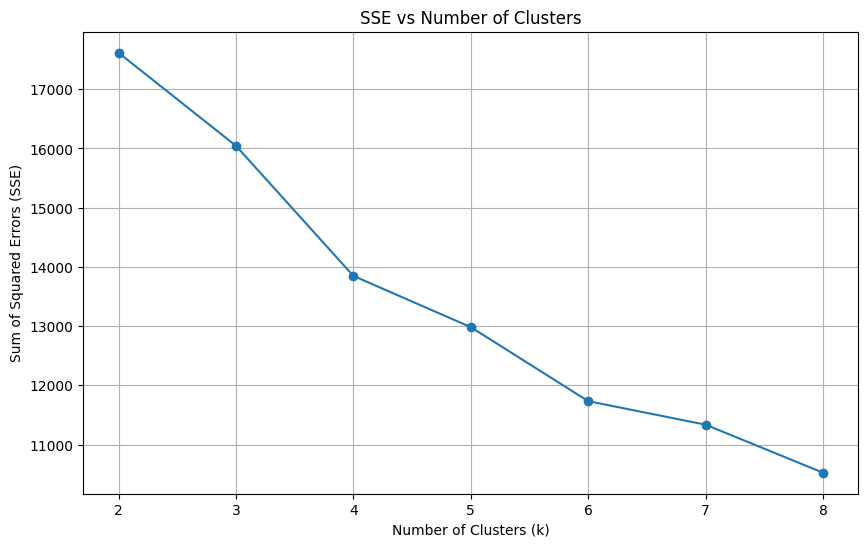
\includegraphics[width=12cm]{./Part II/1_a.png}
            \caption{Sum of squared errors (SSE) according to the number of clusters}
        \end{figure}

        \item \textbf{According to the previous plot, how many underlying customer segments (clusters)
        should there be ? Explain based on the trade off between the clusters and inertia.}

        \vspace{10pt}
        As we can see in the previous plot, Sum of Squared Errors (SSE) decreases as the number of clusters (k) increases which means more clusters lead to better partitioning and lower variance (inertia).
        The highest decrease in SEE is in between k = 2 and k = 4. After that, it becomes more gradual, so there is a lower benefit for adding more clusters. Therefore, we suppose k = 4 is a reasonable number, as it balances the trade-off between cluster complexity and inertia.
        
        \vspace{10pt}
        \item \textbf{Would k-modes be a better clustering approach ? Explain why based on the dataset
        features.}

        \vspace{10pt}
        The dataset contains a mix of categorical features (job, marital, education, default, housing, loan, contact, month, poutcome, and deposit) and numerical features (age, balance, day, duration, campaign, pdays, previous). K-means clustering works by minimizing euclidean distance, which is effective for numerical data but unsuitable for categorical data and since this dataset has more categorical features, k-modes would be a better approach because instead of minimizing variance, it minimizes dissimilarity based on matching categories.
        
    \end{enumerate}

    \item \textbf{Normalize the data using \texttt{StandardScaler}:}
    
    \begin{enumerate}[label=\alph*)]
        \item \textbf{Apply PCA to the data. How much variability is explained by the top 2 components?}
        
        \lstinputlisting[language=Python]{./Part II/2_a.py}

        \vspace{10pt}
        Variability explained by the top 2 components: 22.76\%
        \vspace{10pt}
        
        \item \textbf{Apply \texttt{k-means} clustering with $k=3$ and \texttt{random\_state=42} (all other arguments as default) and use the original 8 features. Next, provide a scatterplot according to the first 2 principal components. Can we clearly separate the clusters? Justify.}
    
        \vspace{10pt}
        \lstinputlisting[language=Python]{./Part II/2_b.py}
        \begin{figure}[H]
            \centering
            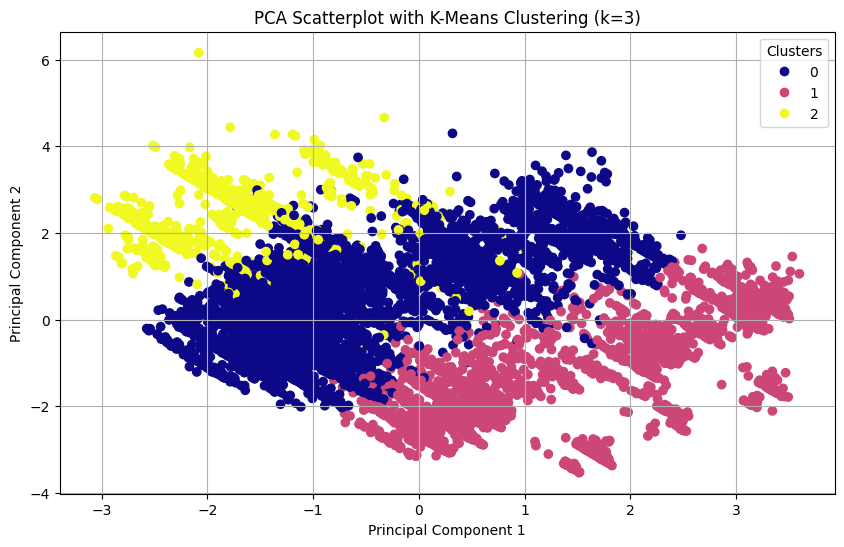
\includegraphics[width=12cm]{./Part II/2_b.png}
            \caption{PCA Scatterplot}
        \end{figure}

        \vspace{10pt}
        Some separation is visible for k-mean clustering with k = 3, but we can't say that they are clearly distinct since there is an overlap, which indicates that these clusters don't have distinct boundaries.
        \vspace{10pt}
        
        \item \textbf{Plot the cluster conditional features of the frequencies of `job" and `education"
        according to k-means, with \texttt{multiple='dodge'}, \texttt{stat='density'},
        \texttt{shrink =0.8}, \texttt{common\_norm=False}. Analyze the frequency plots using \texttt{sns.displot}, (see Data Exploration
        notebook). Describe the main differences between the clusters in no more than half page.}

        \vspace{10pt}
        \lstinputlisting[language=Python]{./Part II/2_c.py}

        \begin{figure}[h]
            \centering
            \captionsetup{font=footnotesize} 
            \begin{minipage}{0.43\textwidth}
                \centering
                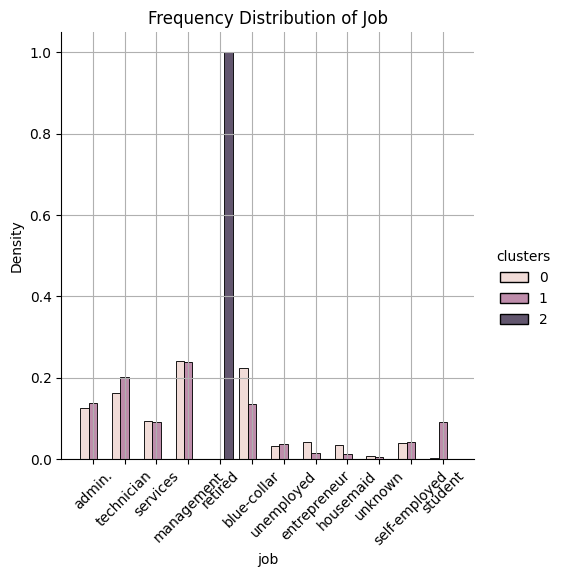
\includegraphics[width=\textwidth]{./Part II/2_c_1.png}
                \caption{Frequency Distribution of Job}
            \end{minipage}
            \begin{minipage}{0.43\textwidth}
                \centering
                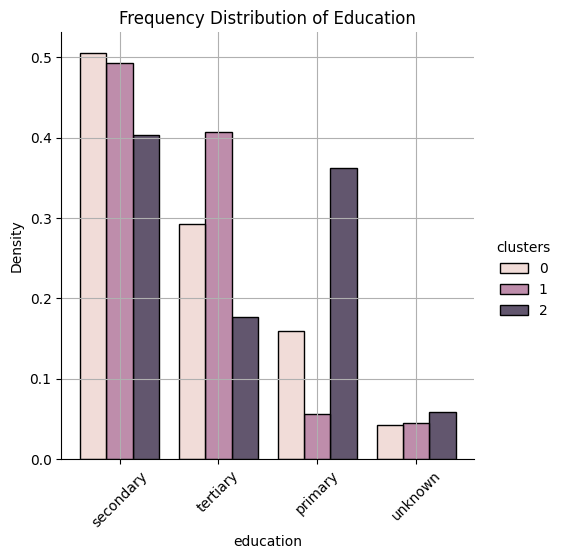
\includegraphics[width=\textwidth]{./Part II/2_c_2.png}
                \caption{Frequency Distribution of Education}
            \end{minipage}
            \caption{Cluster conditional features of the frequencies of `job' and `education'}
        \end{figure}

        \newpage
        \underline{For job frequency distribution:}

        \begin{itemize}
            \item Cluster 0: Has relatively high density in \textbf{management} and \textbf{blue-collar}, which suggests that it is representing workers from a more traditional or stable sector.
            
            \item Cluster 1: Has very low density in \textbf{unemployment}, \textbf{entrepreneur}, \textbf{housemaid}, \textbf{self-employed} and practically zero for \textbf{unknown}. It is highly dense in \textbf{technician}, \textbf{management}, \textbf{blue-color} and \textbf{admin} which let us belive that represents worker from labor sector.
            
            \item Cluster 2: Since has density equal to zero for every job except for \textbf{retired}, it represents retired individuals.
        \end{itemize}

        \vspace{10pt}
        \underline{For education frequency distribution:}
        
        \begin{itemize}
            \item Cluster 0: The highest density value occurs in \textbf{secondary}, always decreasing for the remaining levels 
            (in the order presented above), meaning it represents individuals with mid-level education.
            
            \item Cluster 1: Also has the highest density in \textbf{secondary}, but the value in \textbf{tertiary} is also pretty high. 
            We can notice a large descent for the remaining levels (primary and unknown), these ones having almost the same value 
            between each other. Thus, it represents people with higher-level education.
            
            \item Cluster 2: The highest values of density are found in \textbf{secondary} and \textbf{primary}, which suggests that it is 
            refering to individuals with basic education.
        \end{itemize}
        
        In conclusion, cluster 0 seems to represent people with secondary education who work in blue-color and managment jobs, 
        cluster 1 contains well-educated individuals working mostly on technician and management jobs and cluster 2 consists 
        mainly of people with primary and secondary education, but also having the largest amount of individual in unknown education, 
        who are retired.
        
    \end{enumerate}

\end{enumerate}
\end{document}
